% !TeX program = pdflatex
% Symulator pojazdu elektrycznego do badania ladowarek AC - AMPERE POINT
\documentclass[a4paper,11pt]{article}

\usepackage[utf8]{inputenc}
\usepackage[T1]{fontenc}
\usepackage{lmodern}
\usepackage[polish]{babel}
\usepackage{microtype}
\usepackage[margin=2.3cm]{geometry}
\usepackage{amsmath}
\usepackage{amssymb}
\usepackage{booktabs}
\usepackage{array}
\usepackage{graphicx}
\usepackage{float}
\usepackage{enumitem}
\usepackage{xcolor}
\usepackage[hidelinks]{hyperref}

\newcommand{\ohm}{\,\Omega}
\newcommand{\kohm}{\,\mathrm{k}\Omega}
\newcommand{\Mohm}{\,\mathrm{M}\Omega}
\newcommand{\volt}{\,\mathrm{V}}
\newcommand{\amp}{\,\mathrm{A}}
\newcommand{\watt}{\,\mathrm{W}}
\newcommand{\us}{\,\mu\mathrm{s}}
\newcommand{\ms}{\,\mathrm{ms}}
\newcommand{\sek}{\,\mathrm{s}}

\setlist[itemize]{topsep=2pt,itemsep=1.5pt,parsep=0pt,leftmargin=1.4em}
\setlist[enumerate]{topsep=2pt,itemsep=1.5pt,parsep=0pt,leftmargin=1.8em}

\title{\vspace{-1.5cm}Symulator pojazdu elektrycznego do badania ładowarek AC\\[2mm]
\large Koncepcja i obliczenia --- wydanie 4\\[1mm]
\normalsize wszystko w jednej puszce, tor mocy 3$\times$32~A}
\author{AMPERE POINT}
\date{18 września 2026}

\begin{document}
\maketitle
\thispagestyle{empty}

\noindent\textbf{Schemat:} \texttt{AMPERE\_POINT\_symulator\_pojazdu\_schemat\_v4.pdf}
(wektorowy, do powiększania) oraz \texttt{...\_v4.png} --- wklejony w rozdziale~\ref{sec:schemat}.
Generator: \texttt{generator\_schematu\_v4.py}.

\noindent\textbf{Zastępuje} wydanie~2 w całości. Wydania 1 i~2 zostają w folderze jako historia.
Wszystkie liczby w tym dokumencie są przeliczone od podstaw; miejsca, w których rachunek
zmienił wcześniejsze założenia, są wskazane w dzienniku iteracji (rozdz.~\ref{sec:dziennik}).

\tableofcontents

\section{Po co to urządzenie}

Serwis ma tester z ręcznym przełącznikiem stanów. Taki przyrząd sprawdza ładowarkę
wyłącznie na ścieżce, na której wszystko idzie dobrze: człowiek gałką wymusza stan
ładowania, ładowarka podaje napięcie, wynik jest pozytywny. Prawdziwy samochód robi
coś zupełnie innego --- \textbf{sam decyduje, czy w ogóle zacząć, i potrafi odmówić}.

Przypadek z serwisu, który wymusił tę konstrukcję: ładowarki z wadliwym modułem
zgodności Tesla (zdalne otwieranie klapki) miały przekłamaną rezystancję na linii
obecności wtyku. Samochody odmawiały ładowania. Na ręcznym testerze wszystko
,,działało'', bo stan ładowania wymuszał operator, a nikt nie mierzył rezystancji
kodującej. Wada przechodziła przez kontrolę.

Wniosek konstrukcyjny jest jednoznaczny: \textbf{urządzenie musi odtwarzać proces
decyzyjny samochodu, a nie tylko jego rezystancje.} Stąd cztery cechy, których
tester ręczny nie ma:

\begin{enumerate}
\item po wpięciu wtyku urządzenie \textbf{samo} przechodzi do ładowania --- po
      komplecie sprawdzeń, które robi samochód; gdy cokolwiek się nie zgadza,
      zostaje w stanie ,,podłączony'' i wypisuje powód odmowy;
\item w torze pilota \textbf{nie ma ani jednego ręcznego przełącznika} --- w aucie
      nic nie przełącza się ręką; wszystkie styki zamykają przekaźniki sterowane
      przez mikrokontroler;
\item urządzenie \textbf{mierzy ładowarce czasy}, których wymaga od niej norma
      (podanie i odcięcie napięcia), i wystawia werdykt;
\item tor mocy na pełne \textbf{22~kW (3$\times$32~A)} z gniazdem wyjściowym ---
      pod przyszły magazyn energii albo obciążenie próbne.
\end{enumerate}

\section{Liczby z normy IEC 61851-1}

Cała rozmowa ładowarki z autem przy ładowaniu prądem przemiennym odbywa się na
jednej żyle --- linii pilota sterującego. Ładowarka podaje na nią przez rezystor
$1\kohm$ prostokąt $\pm 12\volt$ o częstotliwości $1$~kHz. Pojazd tylko obciąża tę
linię rezystorami \textbf{przez diodę}, która przewodzi wyłącznie dodatnią połówkę.
Ujemna połówka zostaje nietknięta na $-12\volt$ i po tym ładowarka poznaje, że po
drugiej stronie jest pojazd, a nie zawilgocenie czy przypadkowa rezystancja.

\subsection{Rezystory pojazdu (Tab. A.2)}

Tolerancja wszystkich $\pm 3\%$, spadek na diodzie $0{,}7 \pm 0{,}15\volt$.
Rezystor $2{,}74\kohm$ jest w pojeździe na stałe; styk pojazdu dokłada równolegle
$1{,}3\kohm$ (ładowanie) albo $270\ohm$ (ładowanie z wentylacją):

\[
R_{C}=\frac{2740\cdot 1300}{2740+1300}=881{,}7\ohm,
\qquad
R_{D}=\frac{2740\cdot 270}{2740+270}=245{,}8\ohm .
\]

\subsection{Poziomy stanów (Tab. A.3, okna \texorpdfstring{$\pm 1\volt$}{+/-1 V})}

\begin{center}
\begin{tabular}{llc}
\toprule
Stan & Znaczenie & Szczyt dodatni \\
\midrule
A & brak pojazdu & $+12\volt$ \\
B & pojazd podłączony, nie ładuje & $+9\volt$ \\
C & ładowanie & $+6\volt$ \\
D & ładowanie z wentylacją & $+3\volt$ \\
E & zwarcie pilota do ziemi & $0\volt$ \\
F & ładowarka niesprawna & $-12\volt$ \\
\bottomrule
\end{tabular}
\end{center}

\subsection{Wypełnienie a oferowany prąd (Tab. A.6)}

To jest tabela decyzyjna naszej maszyny. $D$ oznacza wypełnienie w procentach:

\begin{center}
\begin{tabular}{lll}
\toprule
Wypełnienie & Oferta & Decyzja symulatora \\
\midrule
$D<3\%$              & ---                       & ładowanie zabronione \\
$3\% \le D \le 7\%$  & żądanie łącza cyfrowego   & odmowa z komunikatem \\
$7\% < D < 8\%$      & ---                       & zabronione \\
$8\% \le D \le 10\%$ & $6\amp$                   & dopuszczone \\
$10\% < D \le 85\%$  & $I = 0{,}6\amp \cdot D$   & dopuszczone \\
$85\% < D \le 96\%$  & $I = 2{,}5\amp \cdot (D-64)$ & dopuszczone \\
$96\% < D \le 97\%$  & $80\amp$                  & dopuszczone \\
$D>97\%$ lub brak sygnału & ---                  & zabronione \\
\bottomrule
\end{tabular}
\end{center}

Przykład kontrolny dla ładowarki 22~kW: $I=32\amp \Rightarrow D = 32/0{,}6 = 53{,}3\%$.

\subsection{Kodowanie kabla (Tab. B.3)}

Rezystor siedzi we wtyku kabla, między stykiem obecności a ochronnym; tolerancja
$\pm3\%$: $1{,}5\kohm \to 13\amp$; $680\ohm \to 20\amp$; $220\ohm \to 32\amp$;
$100\ohm \to 63\amp$.

\subsection{Czasy (Tab. A.7)}

\begin{center}
\begin{tabular}{llc}
\toprule
Kto & Zdarzenie & Wymaganie \\
\midrule
ładowarka & podanie napięcia po wejściu w stan C & $\le 3\sek$ \\
ładowarka & odcięcie po otwarciu styku pojazdu   & $\le 100\ms$ \\
pojazd    & otwarcie styku, gdy pilot poza tolerancją & $\le 3\sek$ \\
pojazd    & dostosowanie poboru po zmianie wypełnienia & $\le 5\sek$ \\
\bottomrule
\end{tabular}
\end{center}

Dwa pierwsze wiersze symulator \textbf{mierzy i ocenia} (rozdz.~\ref{sec:tester}),
dwa ostatnie \textbf{spełnia} (rozdz.~\ref{sec:maszyna}).

\section{Co już jest w puszce, a co dochodzi}

Konstrukcja mieści się w istniejącej obudowie szczelnej o wymiarach około
$200\times300\times120$~mm, w której jest już zamontowana i okablowana część
wyposażenia. Wykorzystujemy je w całości:

\begin{center}
\begin{tabular}{p{5.2cm}p{10.0cm}}
\toprule
Element istniejący & Rola w tej konstrukcji \\
\midrule
gniazdo wlotowe Type~2 & wlot jak w aucie --- kabel ładowarki wpina się wprost \\
miernik panelowy ,,CP: V DC'' & wskazanie poziomu pilota; dostaje detektor
  szczytu, żeby pokazywał $12/9/6/3\volt$ zamiast średniej z przebiegu
  (rozdz.~\ref{sec:szczyt}) \\
miernik panelowy ,,PP: OHM'' & \textbf{demontowany} --- w jego oknie
  ($\approx 71\times39$~mm) staje wyświetlacz tekstowy $16\times2$
  (potrzebuje $71\times24$~mm, wchodzi bez przerabiania panelu) \\
3 mierniki V/A dla faz & podgląd napięć i prądów niezależny od elektroniki \\
łączniki 16~A na panelu & załączanie zasilania elektroniki \\
gniazdo 230~V & szybkie próby jednofazowe \\
przekładnik prądowy toroidalny, bocznik & pomiar prądu (do sprawdzenia, ile
  przekładników jest w środku --- rozdz.~\ref{sec:otwarte}) \\
\bottomrule
\end{tabular}
\end{center}

\noindent Dochodzi: mikrokontroler z płytką, 5 przekaźników sygnałowych z układem
sterującym cewkami, garść rezystorów i jeden układ komparatora, wyświetlacz
tekstowy, przycisk, brzęczyk, grzybek awaryjny, gniazdo siłowe wyjściowe i przewody
$6$~mm$^2$.

\section{Rdzeń pilota --- gałęzie stanów}

\subsection{Dlaczego rezystor stanu ,,podłączony'' nie ma styku}

Rezystor $2{,}7\kohm$ jest wlutowany na stałe, bez żadnego przełącznika. Tak jest
w aucie: stan ,,podłączony'' powstaje sam z chwilą wpięcia wtyku, bo przed wpięciem
obwód pilota fizycznie nie istnieje --- i to właśnie jest stan ,,brak pojazdu''.
Handlowa wartość mieści się w oknie normy:

\[
2{,}74\kohm \pm 3\% = 2{,}66\ldots2{,}82\kohm,
\qquad
2{,}7\kohm \pm 1\% = 2{,}673\ldots2{,}727\kohm .
\]

\subsection{Pozostałe gałęzie i usterki wstrzykiwane}

\begin{itemize}
\item \textbf{styk pojazdu} (dokłada $1{,}3\kohm$) --- zamykany przez program po
      komplecie sprawdzeń, otwierany przy zatrzymaniu, naruszeniu warunków
      i grzybku awaryjnym;
\item \textbf{gałąź wentylacji} (dokłada $270\ohm$) --- funkcja testowa, większość
      ładowarek tego stanu nie obsługuje;
\item \textbf{zwarcie diody} --- przekaźnik bocznikuje diodę pojazdu; ujemna połówka
      przestaje trzymać $-12\volt$, sprawna ładowarka musi to wykryć i odmówić;
\item \textbf{zanik pojazdu} --- przekaźnik ze stykiem \emph{spoczynkowo zamkniętym}
      w linii pilota; podanie napięcia na cewkę przerywa linię mimo wpiętego wtyku.
      Styk spoczynkowo zamknięty dlatego, że przy braku zasilania elektroniki linia
      pilota ma być ciągła, a nie przerwana;
\item \textbf{zwarcie pilota do ziemi} (stan E) --- prąd zwarcia ogranicza rezystor
      $1\kohm$ w ładowarce:
      \[
      I_{zw}=\frac{12\volt}{1\kohm}=12\ \mathrm{mA},
      \]
      czyli próba jest z założenia bezpieczna dla badanego urządzenia.
\end{itemize}

Cewki pięciu przekaźników sterowane są przez posiadany układ z siedmioma
wzmacniaczami i wbudowanymi diodami gaszącymi.

\subsection{Moc tracona w rezystorach pojazdu}

Najgorszy przypadek to stałe $+12\volt$ na pilocie przy obu zamkniętych gałęziach
(stan D, wypełnienie bliskie 100\%):

\[
P_{max}=\frac{U^2}{R_{D}}=\frac{(12-0{,}7)^2}{245{,}8\ohm}=0{,}52\watt
\]

rozłożone na trzy rezystory. Metalizowane $0{,}6\watt$ z zapasem; praca normalna to
pojedyncze miliwaty, bo prostokąt ma wypełnienie kilkudziesięciu procent, a poziom
w stanie C wynosi $6\volt$:
$P = (6-0{,}7)^2/881{,}7 = 32$~mW.

\subsection{Dlaczego przekaźniki muszą być sygnałowe, a nie mocy}
\label{sec:przekazniki}

To nie jest kwestia gabarytu ani ceny, tylko \textbf{materiału styku}. Przekaźniki
mocy mają styki ze stopu srebra z tlenkiem cyny. Ten materiał jest odporny na
przepalenie łukiem, ale pokrywa się warstwą tlenków i siarczków, którą przebija
dopiero łuk przy załączaniu obciążenia. Producenci podają dla nich minimalne
obciążenie łączeniowe rzędu $100$~mA przy $5\volt$. Poniżej tej granicy styk
\emph{przestaje przewodzić} --- zjawisko znane jako łączenie na sucho.

Prąd, jaki popłynie przez nasz styk w stanie ładowania:

\[
I_{styk}=\frac{U_{CP}-U_{F}}{R_3}=\frac{6-0{,}7}{1300\ohm}=4{,}1\ \mathrm{mA},
\]

czyli \textbf{ponad dwadzieścia razy mniej} niż minimum przekaźnika mocy. Potrzebne
są styki złocone, specyfikowane od mikroamperów i miliwoltów.

Drugi, słabszy argument to rezystancja przejścia. Styk o rezystancji $R_s$ dokłada
się szeregowo do gałęzi $1{,}3\kohm$ i psuje rezystancję wypadkową. Granicę
wyznacza górny kraniec okna $\pm3\%$, czyli $908{,}1\ohm$:

\[
\frac{2740\,(1300+R_s)}{2740+1300+R_s}=908{,}1\ohm
\quad\Longrightarrow\quad
R_s = 58{,}3\ohm .
\]

Styk złocony ma poniżej $100$~m$\Omega$, czyli zapas trzech rzędów wielkości. Ale
uwaga: \textbf{prawdziwym zagrożeniem nie jest ta granica, tylko całkowity brak
przewodzenia} --- styk mocy przy $4$~mA albo przewodzi, albo nie przewodzi wcale,
i żadna wartość pośrednia się nie pojawia.

\section{Tor pomiarowy pilota}
\label{sec:pomiar}

Z jednej żyły trzeba odczytać dwie różne rzeczy. \textbf{Poziom} dodatniej połówki
mówi, w jakim stanie jest połączenie. \textbf{Wypełnienie} mówi, ile prądu
ładowarka oferuje. Poziom mierzy wejście analogowe. Wypełnienia tym samym wejściem
zmierzyć się nie da: pojedyncza konwersja trwa około $100\us$, a okres sygnału to
$1000\us$ --- dziesięć próbek na okres daje błąd rzędu procentów, czyli
kilkudziesięciu setnych ampera. Dlatego drugi tor kończy się komparatorem, który
zamienia przebieg pilota w prostokąt cyfrowy dla licznika sprzętowego.

\subsection{Przesunięcie zakresu \texorpdfstring{$\pm12\volt$}{+/-12 V} w okno
\texorpdfstring{$0\ldots5\volt$}{0...5 V}}

Zwykły dzielnik nie wystarczy, bo potrafi tylko zmniejszać --- z $-12\volt$ zrobi
$-3\volt$, dalej ujemne. Potrzebne jest \emph{dodanie stałej} i po to jest rezystor
podciągający węzeł do $+5\volt$.

\paragraph{Węzeł pomiarowy i co się w nim schodzi.} Cały tor ma jeden punkt,
w którym spotykają się \emph{cztery} drogi --- na schemacie oznaczony literą~A.
Schodzą się w nim:

\begin{center}
\begin{tabular}{clp{7.4cm}}
\toprule
Symbol & Wartość & Dokąd prowadzi \\
\midrule
$R_1$ & $240\kohm$ & do linii pilota (dwa rezystory po $120\kohm$ szeregowo) \\
$R_2$ & $100\kohm$ & do zasilania $+5\volt$ --- to on dodaje stałą \\
$R_3$ & $120\kohm$ & do masy \\
$R_4+R_5$ & $200\kohm$ & do masy przez dzielnik, z którego środka wychodzi sygnał
  do komparatora \\
\bottomrule
\end{tabular}
\end{center}

Dalej: $U_{CP}$ --- napięcie na linii pilota, $U_{zas}=5\volt$, $U_A$ --- szukane
napięcie w tym węźle.

\paragraph{Skąd bierze się wzór.} Ponieważ dróg jest cztery, \textbf{nie wolno użyć
wzoru na zwykły dzielnik napięcia} --- on obowiązuje tylko dla dwóch rezystorów
w szeregu. Trzeba napisać bilans prądów. Prawo prądowe Kirchhoffa mówi, że
\emph{ile prądu do węzła wpływa, tyle z niego wypływa} --- ładunek nigdzie się nie
gromadzi. Prąd w każdej gałęzi liczymy prawem Ohma jako różnicę napięć na jej
końcach podzieloną przez rezystancję. Dwie gałęzie prowadzą do źródeł (pilot
i zasilanie), dwie do masy:

\begin{equation}
\underbrace{\frac{U_{CP}-U_A}{R_1}+\frac{U_{zas}-U_A}{R_2}}_{\text{wpływa do węzła}}
\;=\;
\underbrace{\frac{U_A}{R_3}+\frac{U_A}{R_4+R_5}}_{\text{wypływa do masy}}
\label{eq:bilans}
\end{equation}

Kierunki przyjęte na rysunku są umowne: gdy $U_{CP}$ jest ujemne, pierwszy
składnik po prostu wychodzi ujemny i równanie dalej obowiązuje bez żadnej zmiany.
Teraz wystarczy przenieść wszystko z $U_A$ na jedną stronę:

\[
\frac{U_{CP}}{R_1}+\frac{U_{zas}}{R_2}
= U_A\left(\frac{1}{R_1}+\frac{1}{R_2}+\frac{1}{R_3}+\frac{1}{R_4+R_5}\right)
\]

i podzielić obie strony przez nawias:

\begin{equation}
U_A=\frac{\dfrac{U_{CP}}{R_1}+\dfrac{U_{zas}}{R_2}}
         {\dfrac{1}{R_1}+\dfrac{1}{R_2}+\dfrac{1}{R_3}+\dfrac{1}{R_4+R_5}}
\label{eq:wezelA}
\end{equation}

Mianownik po podstawieniu (w $\mathrm{k}\Omega^{-1}$):

\[
\frac{1}{240}+\frac{1}{100}+\frac{1}{120}+\frac{1}{200}
=0{,}0041\overline{6}+0{,}0100+0{,}008\overline{3}+0{,}0050=0{,}0275
\]

\begin{equation}
\boxed{\;U_A=0{,}1515\,U_{CP}+1{,}818\volt\;}
\label{eq:przelicznik}
\end{equation}

Sprawdzenie krańców i poziomów stanów:

\[
\begin{array}{llll}
U_{CP}=-12\volt \Rightarrow U_A=0{,}00\volt, &
U_{CP}=+3\volt  \Rightarrow U_A=2{,}27\volt, &
U_{CP}=+6\volt  \Rightarrow U_A=2{,}73\volt, \\[1mm]
U_{CP}=+9\volt  \Rightarrow U_A=3{,}18\volt, &
U_{CP}=+12\volt \Rightarrow U_A=3{,}64\volt. & \\
\end{array}
\]

Cały przebieg mieści się w oknie przetwornika i nigdy nie schodzi poniżej zera.
Warto zauważyć, że \textbf{czwarty składnik mianownika to gałąź komparatora} ---
gdyby ją pominąć, współczynnik wyszedłby $0{,}185$ zamiast $0{,}152$. Ta gałąź
obciąża węzeł i musi być w rachunku; wzór na schemacie ją uwzględnia.

\subsection{Ile ten tor obciąża linię pilota}

Prąd pobierany z linii jest największy przy ujemnej połówce, gdy $U_A$ siedzi
na zerze:

\[
I_{CP}=\frac{U_{CP}-U_A}{R_1}=\frac{-12-0}{240\kohm}=-50\ \mu\mathrm{A}.
\]

Ładowarka podaje pilota przez rezystor $1\kohm$, więc zakłócenie poziomu wynosi
$50\,\mu\mathrm{A}\cdot 1\kohm = 0{,}05\volt$ --- dwadzieścia razy mniej niż okno
tolerancji $\pm1\volt$. Pomiar nie przekłamuje tego, co mierzy.

\subsection{Dlaczego diody zabezpieczające nigdy nie przeszkadzają}

Węzeł ma klamrę z dwóch diod: do $+5\volt$ i do masy. Zaczynają przewodzić dopiero
poza zakresem $-0{,}7\ldots5{,}7\volt$. Z równania~\eqref{eq:przelicznik}:

\[
U_A=5{,}7\volt \Rightarrow U_{CP}=+25{,}6\volt,
\qquad
U_A=-0{,}7\volt \Rightarrow U_{CP}=-16{,}6\volt .
\]

Obie granice leżą daleko poza czymkolwiek, co może się pojawić na sprawnej linii,
więc klamra chroni wejście, a przy normalnej pracy jest elektrycznie nieobecna.

\subsection{Rozgałęzienie: droga wygładzona i droga ostra}

Do wejścia analogowego idzie \textbf{droga wygładzona}: $10\kohm$ szeregowo
i $470$~pF do masy tuż przy wejściu. Kondensator pokrywa szarpnięcie, jakie robi
wewnętrzny kondensator próbkujący przetwornika w chwili pomiaru.

Do komparatora odchodzi \textbf{droga ostra}, i to \emph{przed} wygładzaniem.
To nie jest kosmetyka. Gdyby komparator patrzył za kondensatorem, widziałby zbocza
rozmyte stałą czasową $\tau = 10\kohm\cdot470\,\mathrm{pF}=4{,}7\us$, a moment
przekroczenia progu przesuwałby się o ułamek tej stałej. Na okresie $1000\us$
daje to błąd wypełnienia rzędu

\[
\frac{\Delta t}{T}\approx\frac{16\us}{1000\us}=1{,}6\%
\qquad\Rightarrow\qquad
\Delta I = 0{,}6\amp\cdot1{,}6 = 0{,}96\amp,
\]

czyli prawie amper fałszywej oferty. Po rozdzieleniu dróg błąd spada poniżej
$0{,}1\%$.

\subsection{Drugi podział przez dwa}

\begin{equation}
U_B=U_A\cdot\frac{R_5}{R_4+R_5}=\frac{U_A}{2}=0{,}0758\,U_{CP}+0{,}909\volt
\label{eq:wezelB}
\end{equation}

Powód jest twardy. Komparator zasilany napięciem $V_{CC}=5\volt$ gwarantuje
poprawną pracę tylko dla napięć wejściowych poniżej

\[
U_{CM,max}=V_{CC}-1{,}5\volt=3{,}5\volt ,
\]

a $U_A^{max}=3{,}64\volt$ ten limit przekracza. Po podziale
$U_B^{max}=1{,}82\volt$ i jest z dużym zapasem w dozwolonym zakresie.

\subsection{Próg i dlaczego leży akurat tam}

Komparator ma dwa wejścia i mówi wyłącznie, na którym napięcie jest wyższe --- bez
wartości pośrednich. Sygnał z pilota idzie na wejście odwracające, stały próg na
nieodwracające:

\begin{equation}
U_{prog}=5\volt\cdot\frac{10\kohm}{100\kohm+10\kohm}=0{,}4545\volt
\label{eq:prog}
\end{equation}

Przeliczenie progu z powrotem na skalę pilota, z równania~\eqref{eq:wezelB}:

\[
U_{CP}\big|_{prog}=\frac{0{,}4545-0{,}909}{0{,}0758}=-6{,}0\volt .
\]

To jest sedno doboru. Dół prostokąta leży zawsze na $-12\volt$, a najniższa możliwa
góra to $+3\volt$ (stan z wentylacją). Próg siedzi w połowie tego odstępu: $6\volt$
zapasu w dół i $9\volt$ w górę. Żaden stan nie zbliża się do progu.

Skutkiem podania sygnału na wejście odwracające jest \textbf{odwrócenie wyjścia}:
gdy pilot jest na górze, na wyjściu jest zero. Dla pomiaru wypełnienia bez
znaczenia --- program mierzy wtedy czas dolny i odejmuje od stu procent.

\subsection{Rezystor podciągający wyjście}

Wyjście tego komparatora umie tylko ściągać do masy, nie umie podać plusa. Bez
rezystora $10\kohm$ do $+5\volt$ linia wisi w powietrzu i mikrokontroler czyta z niej
przypadkowe stany. To klasyczna pułapka przy tym układzie i osobna pozycja na
liście części.

\subsection{Histereza --- ile i po co}

Blisko progu komparator jest maksymalnie czuły i szum może wywołać serię fałszywych
przeskoków, które licznik sprzętowy policzy jako zbocza. Rezystor $R_8=470\kohm$
z wyjścia na wejście progowe przesuwa próg za każdym przeskokiem w stronę, z której
sygnał przyszedł. Przy $R_6=100\kohm$ do $+5\volt$ i $R_7=10\kohm$ do masy:

\begin{equation}
U_{prog}=\frac{\dfrac{5\volt}{R_6}+\dfrac{U_{wy}}{R_8}}
              {\dfrac{1}{R_6}+\dfrac{1}{R_7}+\dfrac{1}{R_8}}
\label{eq:histereza}
\end{equation}

\[
U_{wy}\approx 4{,}91\volt \Rightarrow U_{prog}=0{,}539\volt,
\qquad
U_{wy}\approx 0\volt \Rightarrow U_{prog}=0{,}446\volt,
\]
\[
\Delta U_{prog}=93\ \mathrm{mV}
\qquad\Longrightarrow\qquad
\Delta U_{CP}=\frac{0{,}093\volt}{0{,}0758}=1{,}23\volt .
\]

W skali pilota próg przeskakuje więc między $-6{,}1\volt$ a $-4{,}9\volt$.
Zakłócenie mniejsze niż $1{,}23\volt$ nie jest w stanie przerzucić wyjścia --- przy
przebiegu o rozpiętości $24\volt$ to około $5\%$ marginesu: dość, by stłumić szum,
za mało, by przesunąć moment przełączenia w mierzalny sposób.

\subsection{Co program z tego liczy}

\begin{equation}
D=\frac{t_H}{t_H+t_L}\cdot100\%,
\qquad
I = 0{,}6\amp\cdot D \quad\text{dla } 10\% < D \le 85\%
\end{equation}

Licznik przy zegarze $16$~MHz i podziale przez $8$ tyka co $0{,}5\us$, więc na
okresie $1000\us$:

\[
\Delta D=\frac{0{,}5\us}{1000\us}=0{,}05\%
\qquad\Longrightarrow\qquad
\Delta I = 0{,}6\amp\cdot0{,}05=0{,}03\amp .
\]

Rozdzielczość toru poziomu, przy przetworniku 10-bitowym i odniesieniu $5\volt$:

\[
\Delta U_{ADC}=\frac{5\volt}{1024}=4{,}88\ \mathrm{mV}
\qquad\Longrightarrow\qquad
\Delta U_{CP}=\frac{4{,}88\ \mathrm{mV}}{0{,}1515}=32\ \mathrm{mV},
\]

czyli trzydzieści razy drobniej niż okno tolerancji stanu. Oba tory wyrastają
z tego samego węzła, więc gdy zaczną pokazywać rzeczy sprzeczne --- na przykład
poziom stanu ładowania przy zerowym wypełnieniu --- to sam w sobie jest sygnał,
że coś jest nie tak albo z ładowarką, albo z naszym układem.

\section{Miernik panelowy pilota --- detektor szczytu}
\label{sec:szczyt}

Istniejący miernik panelowy podpięty wprost do linii pilota pokazywałby wartość
średnią z prostokąta, czyli liczbę zależną od wypełnienia, a nie od stanu. Żeby
pokazywał to, co ma pokazywać --- $12/9/6/3\volt$ --- dostaje prosty detektor
szczytu: rezystor szeregowy $R_s$, dioda i kondensator $C$ na wejściu miernika.

Rozmiary tych trzech elementów wynikają z dwóch błędów, które trzeba zmieścić
w oknie $\pm1\volt$ z tabeli stanów. Niech $R_{we}$ będzie rezystancją wejściową
miernika, $T=1\ms$ okresem, $D$ wypełnieniem.

\paragraph{Opadanie między impulsami.} Kondensator rozładowuje się przez wejście
miernika przez cały czas trwania dolnej połówki:

\begin{equation}
\Delta U_{op}\approx\frac{U\,T}{R_{we}\,C}
\label{eq:opadanie}
\end{equation}

\paragraph{Spadek na rezystorze szeregowym.} Ładunek utracony w okresie musi zostać
uzupełniony w czasie górnej połówki $t_H = D\,T$. Ładunek to
$\Delta Q = C\,\Delta U_{op} = U T/R_{we}$, więc średni prąd doładowania wynosi
$\Delta Q/t_H$, a spadek na rezystorze:

\begin{equation}
\Delta U_{sz}=R_s\cdot\frac{\Delta Q}{t_H}=\frac{R_s}{R_{we}}\cdot\frac{U}{D}
\label{eq:szereg}
\end{equation}

Pojemność się skróciła --- spadek na rezystorze od niej nie zależy, zależy tylko od
stosunku rezystancji i od wypełnienia. Najgorszy przypadek to najmniejsze
dopuszczalne wypełnienie, $D=0{,}10$.

\paragraph{Dobór.} Przyjmując budżet $0{,}3\volt$ na każdy z dwóch błędów,
$U=12\volt$ i zakładaną $R_{we}=1\Mohm$:

\[
R_s \le \frac{R_{we}\,D_{min}\,\varepsilon}{U}
     = \frac{10^6\cdot0{,}10\cdot0{,}3}{12}=2{,}5\kohm
\quad\Rightarrow\quad R_s = 2{,}2\kohm,
\]
\[
C \ge \frac{U\,T}{R_{we}\,\varepsilon}
   = \frac{12\cdot10^{-3}}{10^{6}\cdot0{,}3}=40\ \mathrm{nF}
\quad\Rightarrow\quad C = 100\ \mathrm{nF}.
\]

Trzeci błąd to spadek na diodzie --- systematyczny i zawsze w tę samą stronę.
Dioda krzemowa zabiera $0{,}7\volt$, dioda Schottky'ego typu BAT85 około
$0{,}25\volt$ przy tych prądach. Bilans najgorszego przypadku ($D=10\%$):

\[
0{,}25 + 0{,}26 + 0{,}06 = 0{,}57\volt < 1\volt ,
\]

czyli \textbf{błąd wskazania mieści się wewnątrz okna tolerancji, jakie sama norma
daje poziomom stanów} --- miernik nigdy nie pokaże jednego stanu jako innego.
Z diodą krzemową bilans wyszedłby $1{,}02\volt$, czyli poza oknem; stąd Schottky.

\paragraph{Warunek do sprawdzenia.} Cały rachunek stoi na założeniu
$R_{we}=1\Mohm$. \textbf{Rezystancję wejściową istniejącego miernika trzeba
zmierzyć} (rozdz.~\ref{sec:otwarte}). Gdyby wyszła $100\kohm$, ze
wzorów~\eqref{eq:opadanie} i~\eqref{eq:szereg} wynika $R_s=220\ohm$
i $C=1\,\mu\mathrm{F}$ --- te same wzory, inne wartości.

\section{Tor obecności wtyku i kodowania kabla}

Prosty dzielnik: $+5\volt$ przez $1\kohm$ na styk obecności, z którego rezystor
kodujący idzie do ziemi. Mierzone napięcie:

\begin{equation}
U_{PP}=5\volt\cdot\frac{R_{PP}}{R_{PP}+1\kohm}
\end{equation}

\begin{center}
\begin{tabular}{lccc}
\toprule
Kabel & $R_{PP}$ & $U_{PP}$ & Okno przy $\pm3\%$ \\
\midrule
brak kabla (rozwarcie) & $\infty$        & $5{,}000\volt$ & --- \\
$13\amp$               & $1{,}5\kohm$    & $3{,}000\volt$ & $2{,}963\ldots3{,}035\volt$ \\
$20\amp$               & $680\ohm$       & $2{,}024\volt$ & $1{,}987\ldots2{,}060\volt$ \\
$32\amp$               & $220\ohm$       & $0{,}902\volt$ & $0{,}886\ldots0{,}924\volt$ \\
$63\amp$               & $100\ohm$       & $0{,}455\volt$ & $0{,}442\ldots0{,}467\volt$ \\
zwarcie                & $0$             & $0{,}000\volt$ & --- \\
\bottomrule
\end{tabular}
\end{center}

Najciaśniejsza para sąsiadów to $32\amp$ i $63\amp$: odstęp $0{,}42\volt$ przy
szerokości okien po $0{,}04\volt$ i rozdzielczości przetwornika $4{,}88$~mV.
Rozróżnienie jest pewne z zapasem rzędu dziesięciokrotnego.

\textbf{To jest tor, który wyłapuje przypadek z rozdziału~1.} Wartość poza każdym
z okien oznacza wadliwy kabel albo wadliwy moduł w ładowarce, symulator zostaje
w stanie ,,podłączony'' i wypisuje zmierzoną rezystancję. Ręczny tester tego nie
pokazuje, bo nie ma czego porównać z tabelą.

\section{Maszyna decyzyjna}
\label{sec:maszyna}

\subsection{Warunki zamknięcia styku pojazdu}

Wszystkie naraz, sprawdzane w sposób ciągły:

\begin{enumerate}
\item rezystancja kodująca kabla mieści się w jednym z okien tabeli; poza nimi ---
      odmowa z podaniem wartości;
\item sygnał sterujący jest obecny, a wypełnienie leży w dozwolonym przedziale
      (w tym strefy zakazane $7\ldots8\%$ i powyżej $97\%$); wypełnienie
      $3\ldots7\%$ to żądanie łącza cyfrowego --- odmowa z komunikatem;
\item poziomy pilota mieszczą się w oknach $\pm1\volt$; poza oknem --- odmowa
      z podaniem zmierzonego poziomu;
\item upłynęło opóźnienie startu (nastawne $0\ldots10\sek$, domyślnie $2\sek$ ---
      odpowiednik automatyki startu w autach);
\item przycisk zatrzymania nie jest wciśnięty, grzybek awaryjny zwolniony.
\end{enumerate}

\subsection{Przebieg sesji}

Wpięcie wtyku $\rightarrow$ stan ,,podłączony'' powstaje sam $\rightarrow$
sprawdzenia $\rightarrow$ zamknięcie styku pojazdu $\rightarrow$ stan ,,ładowanie''
$\rightarrow$ pomiar czasu podania napięcia $\rightarrow$ nadzór ciągły
(wypełnienie, poziomy, kodowanie kabla, pobór prądu kontra oferta; zmiana
wypełnienia $\rightarrow$ nowy limit i komunikat) $\rightarrow$ zatrzymanie albo
naruszenie warunków $\rightarrow$ otwarcie styku w czasie $\le 3\sek$, jak każe
norma $\rightarrow$ pomiar czasu odcięcia.

\subsection{Kierunek bezpieczny}

\textbf{Brak zasilania elektroniki oznacza wszystkie przekaźniki opadnięte, czyli
stan ,,podłączony'', czyli ładowarka nie podaje napięcia.} Grzybek awaryjny
rozcina zasilanie cewek sprzętowo, bez udziału programu --- po jego wciśnięciu
styk pojazdu otwiera się natychmiast, a ładowarka ma obowiązek odciąć napięcie
w $\le100\ms$. To jest ta sama droga, którą i tak badamy, więc grzybek jednocześnie
wyzwala i sprawdza.

\section{Rola testera --- co mierzymy ładowarce}
\label{sec:tester}

Trzy izolowane detektory obecności napięcia (transoptor za mostkiem, każda faza
względem przewodu neutralnego) stoją \textbf{przed} gniazdem wyjściowym, więc widzą
napięcie ładowarki niezależnie od tego, co jest do gniazda podłączone. Z nich:

\begin{itemize}
\item \textbf{czas podania napięcia} --- od zamknięcia styku pojazdu do pojawienia
      się napięcia; wynik pozytywny przy $\le3\sek$;
\item \textbf{czas odcięcia} --- od otwarcia styku pojazdu do zaniku napięcia;
      wynik pozytywny przy $\le100\ms$. Ten pomiar wykrywa między innymi sklejony
      stycznik w ładowarce;
\item \textbf{konfiguracja faz} --- które fazy są obecne; auta z modułową ładowarką
      pokładową ładują z jednej do trzech faz, więc raport z tego jest osobną
      wartością diagnostyczną.
\end{itemize}

Prądy trzech faz mierzą przekładniki dzielone, każdy przez tor dopasowujący:
obciążnik plus podniesienie punktu spoczynkowego do $2{,}5\volt$ (dzielnik
$2\times10\kohm$ z $+5\volt$ i kondensator odsprzęgający), bo przetwornik mierzy
$0\ldots5\volt$, a sygnał przekładnika jest przemienny wokół zera. Wartość
skuteczną liczy program. Zastosowanie: pilnowanie, czy pobór nie przekracza oferty,
oraz asymetria faz.

\section{Tor mocy 3\texorpdfstring{$\times$}{x}32~A}

\subsection{Dlaczego w puszce nie ma zabezpieczeń}

Ładowarka jest wpinana do istniejącej rozdzielnicy biurkowej, która ma własne
zabezpieczenia 32~A i \textbf{nie jest przerabiana}. Sama badana ładowarka ma
własne zabezpieczenie różnicowoprądowe $30$~mA z detekcją $6$~mA prądu stałego
i własny wyłącznik mocy. Te elementy pracują \emph{szeregowo} z naszym obwodem,
więc drugi komplet w puszce niczego nie dodaje --- a w jednym przypadku wręcz
szkodzi: \textbf{drugie zabezpieczenie różnicowoprądowe $30$~mA zadziałałoby przed
zabezpieczeniem badanej ładowarki i zamaskowało wynik jej badania.}

Warunek, który z tego wynika: \textbf{przekrój żył w puszce musi odpowiadać
zabezpieczeniu w rozdzielnicy} --- $32\amp \Rightarrow 6$~mm$^2$. Zabezpieczenie
nadprądowe chroni przewód, a nie urządzenie, więc to jedyne, czego nie wolno tu
uprościć.

\subsection{Bilans cieplny}

Rezystywność miedzi w temperaturze pracy $70\,^\circ$C:

\[
\rho = 0{,}0175\cdot\left(1+0{,}00393\cdot50\right)
     = 0{,}0209\ \frac{\Omega\cdot\mathrm{mm}^2}{\mathrm{m}} .
\]

Droga w puszce na fazę około $0{,}6$~m przy przekroju $6$~mm$^2$:

\[
R_{\ell}=\frac{\rho\,\ell}{A}=\frac{0{,}0209\cdot0{,}6}{6}=2{,}09\ \mathrm{m}\Omega,
\qquad
P_{\ell}=I^2R_{\ell}=32^2\cdot2{,}09\cdot10^{-3}=2{,}14\watt
\]

na fazę, czyli $6{,}4\watt$ w przewodach. Zaciski: około czterech połączeń
śrubowych na fazę po $0{,}15$~m$\Omega$:

\[
P_{z}=3\cdot32^2\cdot4\cdot0{,}15\cdot10^{-3}=1{,}84\watt .
\]

Razem $P\approx 8{,}3\watt$. Powierzchnia obudowy:

\[
A_{ob}=2(0{,}2\cdot0{,}3)+2(0{,}2\cdot0{,}12)+2(0{,}3\cdot0{,}12)=0{,}24\ \mathrm{m}^2 .
\]

Przy współczynniku przejmowania ciepła $h=4\ldots5{,}5$~W/(m$^2\cdot$K) dla obudowy
z tworzywa:

\[
\Delta T=\frac{P}{h\,A_{ob}}=\frac{8{,}3}{(4\ldots5{,}5)\cdot0{,}24}=6\ldots9\ \mathrm{K}.
\]

Przy otoczeniu $30\,^\circ$C daje to wewnątrz $36\ldots39\,^\circ$C --- bezpiecznie
poniżej wytrzymałości obudowy i elektroniki.

\textbf{Ale nie przewody są tu ryzykiem, tylko styki.} Jeden luźny zacisk
o rezystancji $5$~m$\Omega$ wydziela

\[
P = 32^2\cdot5\cdot10^{-3}=5{,}1\watt
\]

\emph{w jednym punkcie} --- tyle, ile cała reszta toru razem wzięta, na powierzchni
kilku milimetrów kwadratowych. Stąd wymóg: końcówki tulejkowe na każdej żyle
i dokręcenie kluczem dynamometrycznym momentem podanym przez producenta listwy,
a po pierwszej sesji obciążeniowej kontrola temperatury zacisków.

\subsection{Wyjście}

Przelot z wlotu przez listwę zaciskową i przekładniki prądowe wprost do gniazda
siłowego $32\amp$ (nowe) i --- odgałęzieniem fazy pierwszej z przewodem
neutralnym --- do istniejącego gniazda $230\volt$. Przewód ochronny idzie prosto
ze styku wlotu do obu gniazd i \textbf{nigdzie nie jest przełączany}.

\subsection{Ograniczenie przyjęte świadomie}

Symulator \textbf{nie ma własnego rozłącznika mocy}. Jeżeli badana ładowarka nie
odetnie napięcia mimo zgłoszenia końca ładowania --- czyli dokładnie wtedy, gdy
jest wadliwa --- urządzenie wykrywa to detektorami faz, pokazuje błąd i włącza
brzęczyk, a odcięcia dokonuje operator wyłącznikiem w rozdzielnicy. Sesje prowadzi
technik obecny przy stanowisku, więc droga reakcji jest krótka; dołożenie własnego
stycznika 3-fazowego $40\amp$ do tej obudowy oznaczałoby rezygnację z części
istniejącego wyposażenia.

\section{Magazyn energii --- samochód bez baterii}

Symulator kończy się tam, gdzie w aucie zaczyna się ładowarka pokładowa: przy
przetwornicy prądu przemiennego na stały, która w aucie jest osobnym modułem za
stykami. \textbf{Konwersję wykonuje ładowarka magazynu wpięta w gniazdo siłowe},
a symulator dostarcza całą resztę auta --- stany, sprawdzenia, limit prądu
odczytany z wypełnienia (pokazywany i pilnowany przekładnikami).

Argument przeciw wbudowaniu przetwornicy $22$~kW: koszt wielokrotnie przewyższający
resztę urządzenia, masa i chłodzenie klasy szafy, brak certyfikacji --- przy zerowym
zysku wierności symulacji, bo \textbf{ładowarka widzi wyłącznie pobierany prąd, nie
to, co się z nim dzieje dalej}. Architektura modułowa daje przy tym elastyczność:
dziś grzałka w gnieździe $230\volt$ jako obciążenie próbne, jutro prostowniki
i bateria w gnieździe siłowym --- bez żadnej zmiany w symulatorze.

\section{Zasilanie elektroniki i bezpieczeństwo pracy}

Elektronika żyje z zasilacza $5\volt$ zasilanego z rozdzielnicy cienkim przewodem
prowadzonym poza torem mocy --- odpowiednik instalacji $12\volt$ w aucie, która
działa, zanim pojawi się jakiekolwiek ładowanie. Dzięki temu komunikaty
i sprawdzenia działają w stanach ,,brak pojazdu'' i ,,podłączony'', zanim ładowarka
poda napięcie.

\begin{itemize}
\item w stanie ładowania gniazda wyjściowe są pod napięciem $230/400\volt$ do
      $32\amp$ na fazę; praca wyłącznie przy zamkniętej obudowie;
\item przed otwarciem obudowy: zatrzymanie, wypięcie wtyku, kontrola braku napięcia;
\item po montażu, przed pierwszym wpięciem w ładowarkę: ciągłość przewodu ochronnego
      od styku wlotu do bolców obu gniazd, brak ciągłości między fazami a ochronnym,
      próba progów sprawdzeń na znanych rezystorach;
\item obciążenie dołączane do gniazd $\le$ oferta pokazana na wyświetlaczu
      i $\le 32\amp$;
\item wszystkie sprzężenia z torem mocy są izolowane: transoptory i przekładniki
      prądowe.
\end{itemize}

\section{Ograniczenia przyjęte świadomie}

\begin{itemize}
\item bez łącza cyfrowego (ISO 15118) --- wypełnienie $5\%$ jest wykrywane
      i komunikowane, nie obsługiwane; serwisowane serie pracują analogowo;
\item bez siłownika blokady wtyku --- ładowarki nie weryfikują blokady po stronie
      pojazdu, zatrzask mechaniczny gniazda wystarcza;
\item pomiar prądu klasy diagnostycznej (przekładniki dzielone, przetwornik
      10-bitowy), nie rozliczeniowej;
\item detektory faz mierzą obecność napięcia, nie jego jakość --- zapady i kształt
      przebiegu są poza zakresem tego urządzenia;
\item brak własnego rozłącznika mocy (uzasadnienie wyżej);
\item stan ,,ładowarka niesprawna'' rozpoznawany po zaniku dodatniej połówki przy
      zachowanej ujemnej, bez osobnego toru pomiaru ujemnego szczytu.
\end{itemize}

\section{Wybór mikrokontrolera}

Rodzina ATmega328 zasilana $5\volt$, a nie układ $3{,}3\volt$ --- z trzech powodów,
z których każdy jest liczbą:

\begin{enumerate}
\item cała sieć pomiarowa z równania~\eqref{eq:przelicznik} jest odniesiona do
      $5\volt$; przy zasilaniu $3{,}3\volt$ trzeba przeliczyć wszystkie cztery
      rezystory węzła i próg komparatora, a zapas do granicy zakresu wejściowego
      komparatora ($V_{CC}-1{,}5\volt = 1{,}8\volt$) zrobiłby się niebezpiecznie
      mały;
\item wejście przechwytywania licznika sprzętowego jest fizycznie na wyprowadzeniu
      D8 --- dokładnie tam, gdzie prowadzi wyjście komparatora; pomiar wypełnienia
      dzieje się wtedy w sprzęcie, bez udziału programu;
\item spójność z rejestratorem złącza --- ta sama sieć pomiarowa, te same wzory,
      te same części, wzajemna weryfikacja obu przyrządów.
\end{enumerate}

Rozdział wyprowadzeń: D2--D4 detektory faz, D5 przycisk, D6 brzęczyk, D7 styk
pojazdu, D8 komparator, D9--D12 gałąź wentylacji i trzy usterki wstrzykiwane,
A1 poziom pilota, A2 kodowanie kabla, A3/A6/A7 prądy faz, A4/A5 wyświetlacz.
Wszystko mieści się bez kompromisów, z jednym wolnym wejściem analogowym.

\section{Schemat}
\label{sec:schemat}

\begin{figure}[H]
\centering
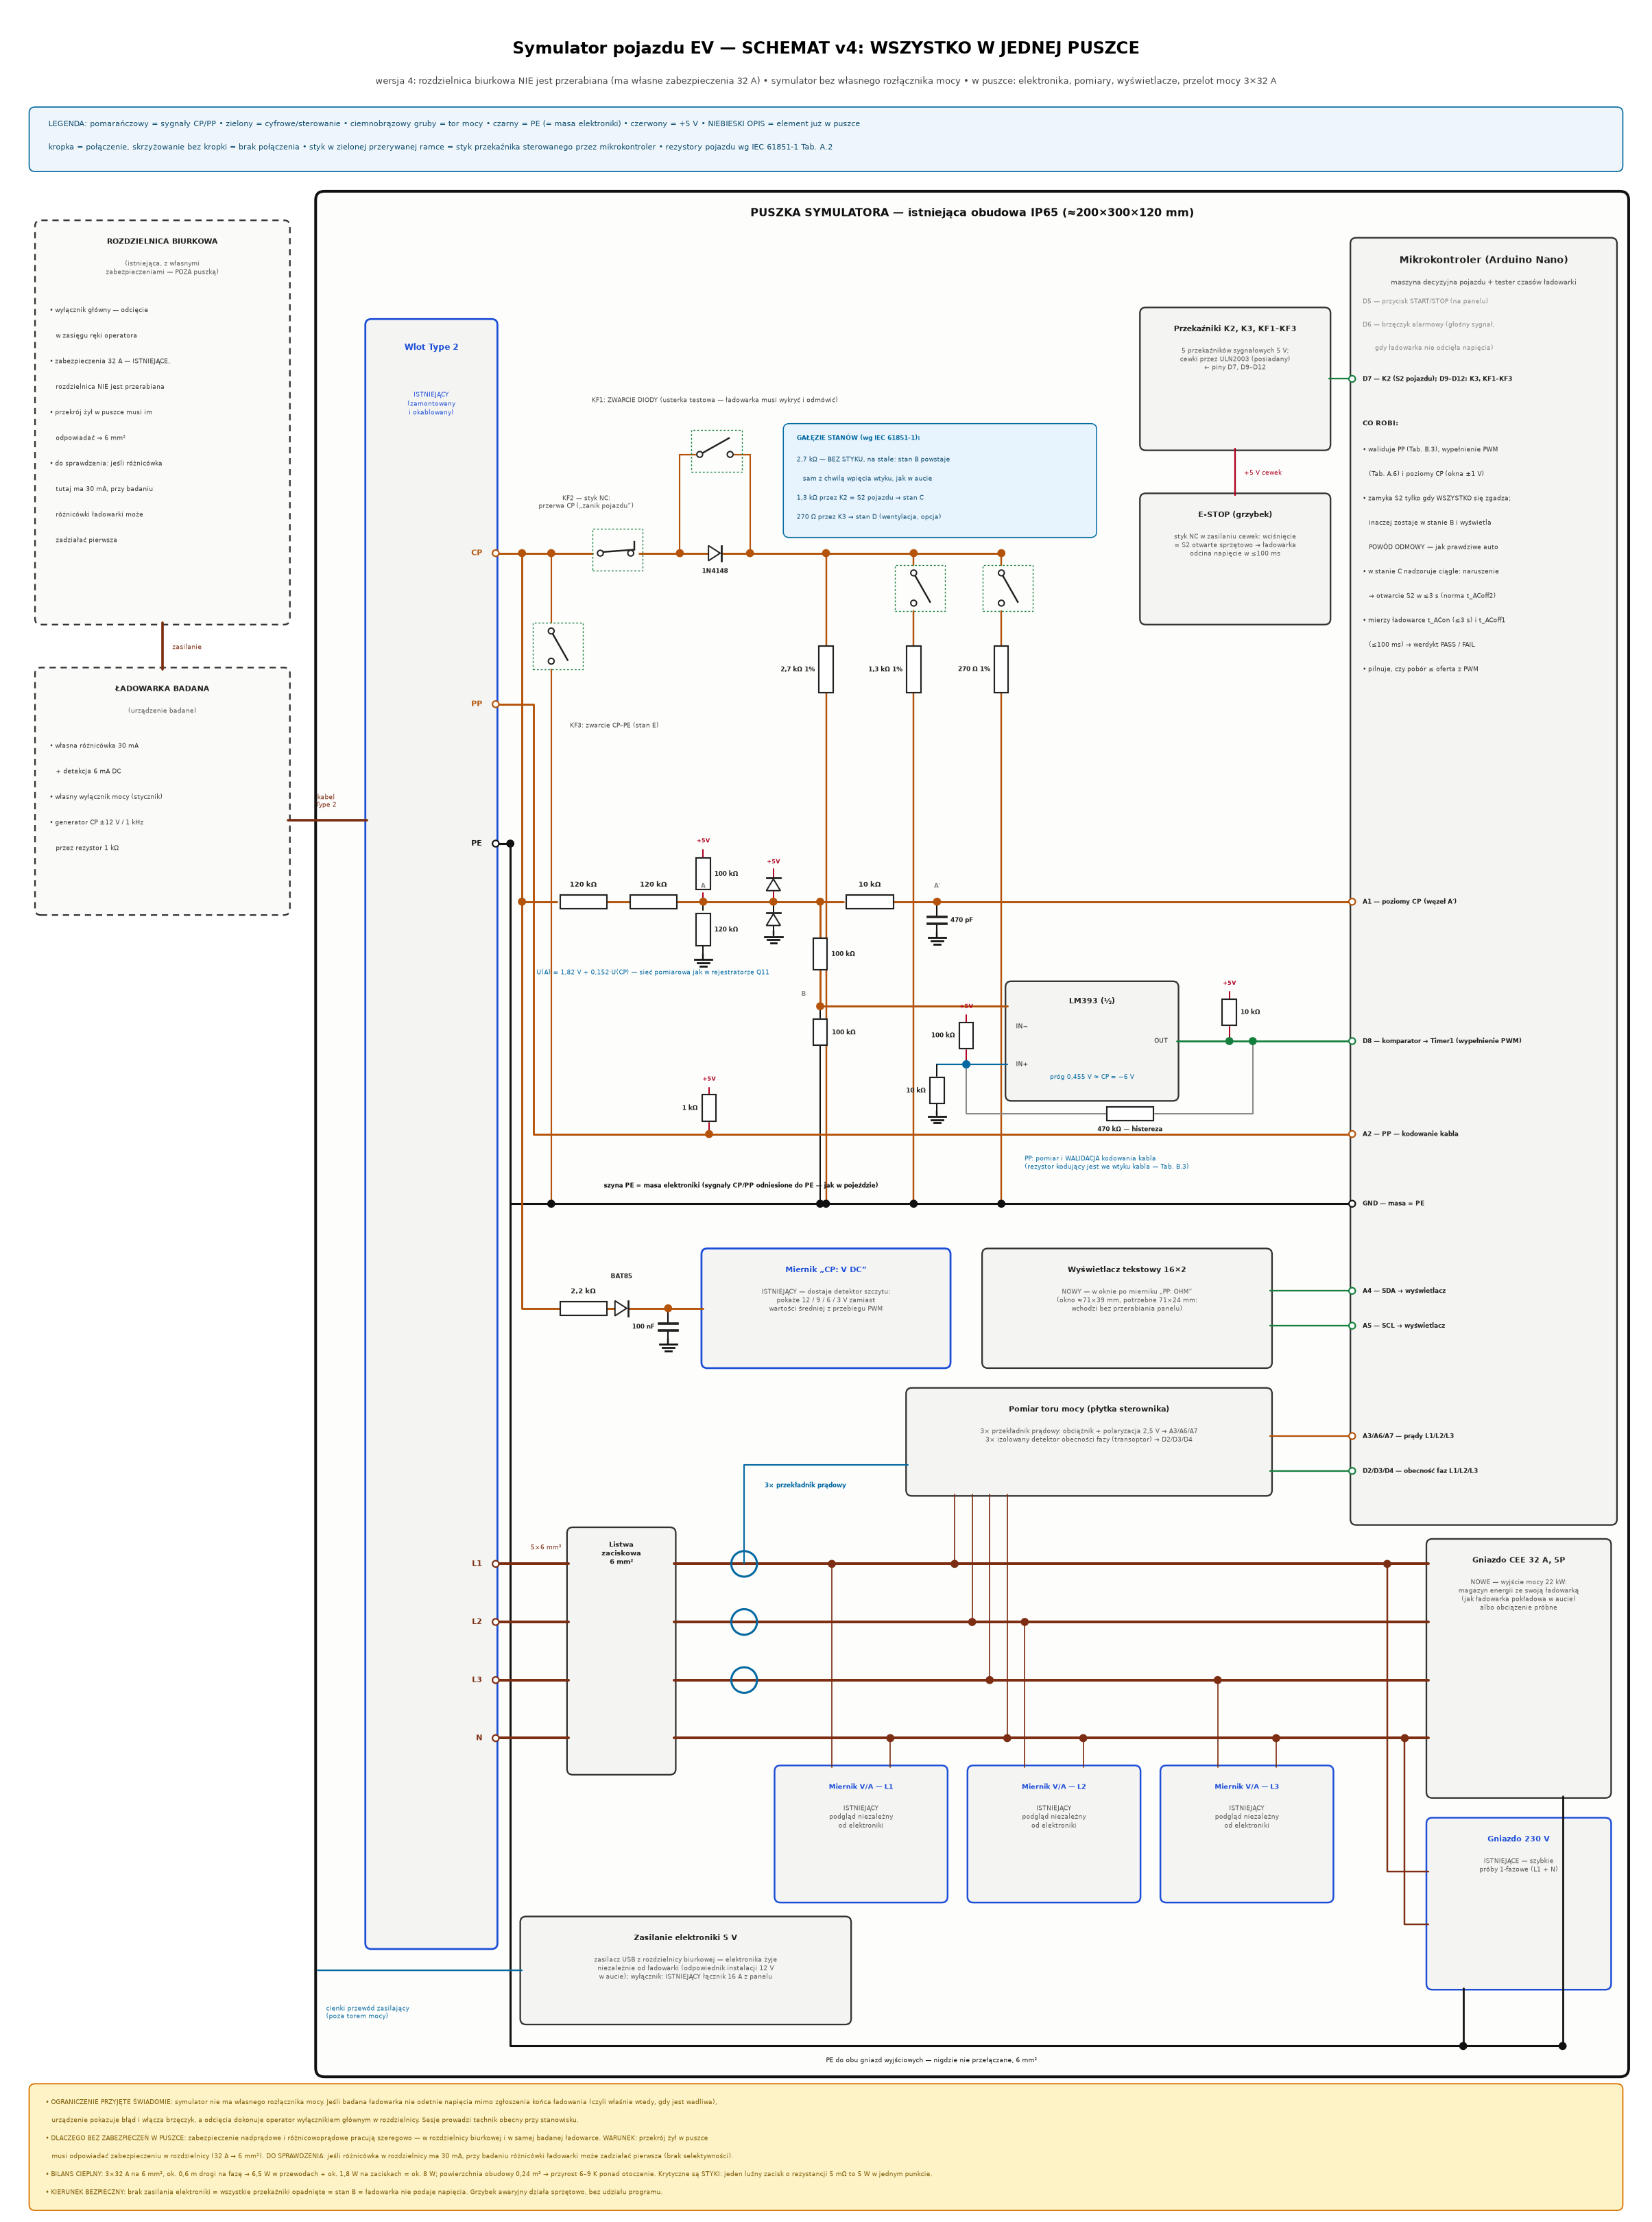
\includegraphics[width=\textwidth]{AMPERE_POINT_symulator_pojazdu_schemat_v4.png}
\caption{Symulator pojazdu EV --- schemat v4. Wersja wektorowa (PDF) pozwala
powiększać dowolny fragment.}
\end{figure}

\section{Co trzeba zmierzyć i otwarte kwestie}
\label{sec:otwarte}

\paragraph{Pomiary na istniejącej puszce (blokują ostateczną listę części).}
\begin{enumerate}
\item wymiary wewnętrzne obudowy oraz okno pozostałe po zdemontowanym mierniku
      rezystancji --- sprawdzenie, czy wyświetlacz $16\times2$ wchodzi bez
      przerabiania panelu;
\item obciążalność zamontowanego wlotu Type~2: $16\amp$ czy $32\amp$ --- przy
      $16\amp$ cały tor mocy trzeba przeprojektować na mniejszy prąd albo wymienić
      wlot;
\item dokąd prowadzi czarny przewód wychodzący przez dławnicę;
\item ile przekładników prądowych jest w środku --- potrzebne są trzy;
\item \textbf{rezystancja wejściowa miernika panelowego pilota} --- od niej zależą
      wartości z rozdziału~\ref{sec:szczyt};
\item ile faz podaje rozdzielnica biurkowa i jaką ma czułość zabezpieczenie
      różnicowoprądowe (przy $30$~mA brak selektywności wobec ładowarki;
      właściwe jest $100$~mA typu A).
\end{enumerate}

\paragraph{Do rozstrzygnięcia.}
\begin{itemize}
\item płytka z mikrokontrolerem w zamówieniu jest w wersji bez gniazda USB ---
      wymaga przejściówki USB--UART z wyprowadzonym sygnałem resetu albo wymiany
      na wersję z wbudowanym USB;
\item raster złącza taśmowego zmierzony suwmiarką wyszedł około $1{,}8$~mm, co nie
      jest wartością znormalizowaną. Metoda rozstrzygająca: zmierzyć odległość
      \emph{od środka pierwszego do środka dziesiątego styku} (dziewięć odstępów);
      $18{,}0$~mm oznacza raster $2{,}0$~mm, $22{,}9$~mm oznacza $2{,}54$~mm.
      Przy $2{,}0$~mm części nie pasują do płytek uniwersalnych o rastrze
      $2{,}54$~mm --- dotyczy to również rejestratora złącza;
\item dokładne treści komunikatów na wyświetlaczu i lista scenariuszy sekwencji
      automatycznej;
\item format zapisu sesji przez USB --- wspólny z rejestratorem złącza.
\end{itemize}

\section{Dziennik iteracji}
\label{sec:dziennik}

\paragraph{Iteracja 1 (3 IX 2026, wydanie 1).} Rdzeń stanów czysto sprzętowy
z ręcznym przełącznikiem obrotowym, elektronika tylko obserwująca, tor $16\amp$.
Odrzucony w całości: powtarzał wadę testera ręcznego.

\paragraph{Iteracja 2 (11 IX 2026, wydanie 2).} Przebudowa na aktywną maszynę
decyzyjną: urządzenie samo przechodzi do ładowania i potrafi odmówić; z toru pilota
usunięto wszystkie ręczne przełączniki; usterki wstrzykiwane przekaźnikami; dodana
rola testera czasów; tor mocy podniesiony do $22$~kW; magazyn energii
w architekturze modułowej.

\paragraph{Iteracja 3 (17 IX 2026, schemat v3).} Koncepcja jednej puszki
z propozycją przeróbki rozdzielnicy. Zachowana w folderze bez zmian na żądanie
użytkownika.

\paragraph{Iteracja 4 (17--18 IX 2026, to wydanie).} Rozdzielnica biurkowa nie jest
przerabiana --- ma własne zabezpieczenia $32\amp$; w puszce nie ma zabezpieczeń
(argument szeregowości i maskowania badanego zabezpieczenia
różnicowoprądowego), zamiast rozłącznika mocy brzęczyk i ograniczenie przyjęte
świadomie. Poprawki wykryte przy przeliczaniu wszystkiego od podstaw:

\begin{enumerate}
\item \textbf{dioda pojazdu była podłączona tylko z jednej strony} --- na rysunku
      brakowało odcinka między węzłem gałęzi usterkowej a anodą, więc przez diodę
      nic by nie płynęło. Poprawione;
\item \textbf{zgubiony rezystor histerezy} $470\kohm$ --- istniał w starszym
      generatorze, zniknął przy przepisywaniu. Przywrócony wraz z drogą sprzężenia;
      liczby w rozdziale~\ref{sec:pomiar} są policzone dla przywróconego układu;
\item \textbf{detektor szczytu przy mierniku panelowym był źle dobrany} ---
      rezystor $100\kohm$ przy zakładanej rezystancji wejściowej miernika $1\Mohm$
      daje ze wzoru~\eqref{eq:szereg} spadek $1{,}2\volt$ przy najmniejszym
      wypełnieniu, czyli wskazanie wychodziło poza okno tolerancji stanu.
      Zmienione na $2{,}2\kohm$; dioda krzemowa zamieniona na Schottky'ego
      (bilans $0{,}57\volt$ zamiast $1{,}02\volt$);
\item \textbf{bilans cieplny przeliczony} --- wcześniejsza nota mówiła
      o $15\watt$ i przyroście $12\ldots15$~K; rachunek z rezystywnością miedzi
      w temperaturze pracy daje $8{,}3\watt$ i $6\ldots9$~K. Nota na schemacie
      poprawiona, wniosek bez zmian: ryzykiem są styki, nie przewody;
\item \textbf{współczynnik przelicznika węzła pomiarowego zweryfikowany} ---
      $0{,}1515$ jest poprawne \emph{pod warunkiem} uwzględnienia gałęzi
      komparatora w mianowniku równania~\eqref{eq:wezelA}; bez niej wyszłoby
      $0{,}185$. Wzór na schemacie jest zgodny z rysowanymi wartościami.
\end{enumerate}

\end{document}
